\documentclass{article}

% Package `amsthm` and `thmtools` must come before package `hyperref`.
\usepackage{amsthm}
\usepackage{thmtools}
% Package `hyperref` must come before package `complexity`.
\usepackage[pdftitle={Complexity of computing the size of the minimum generating set of a group}, pdfauthor={Jeffrey Finkelstein}]{hyperref}
\usepackage{complexity}
\usepackage{amsmath}
\usepackage{amssymb}
\usepackage{tikz}

\newcommand{\gen}[1]{{\langle #1 \rangle}}
\newcommand{\email}[1]{\href{mailto:#1}{\nolinkurl{#1}}}
\newcommand{\AND}{\textsc{and}}
\newcommand{\OR}{\textsc{or}}
\newcommand{\NOT}{\textsc{not}}
\newcommand{\pair}[2]{\left\langle #1, #2 \right\rangle}
\newcommand{\triple}[3]{\left\langle #1, #2, #3 \right\rangle}

\declaretheorem[numberwithin=section]{theorem}
\declaretheorem[numberlike=theorem]{conjecture}
\declaretheorem[numberlike=theorem]{lemma}
\declaretheorem[numberlike=theorem]{proposition}
\declaretheorem[numberlike=theorem, style=definition]{definition}
\declaretheorem[numberlike=theorem, style=definition]{todo}

\title{Complexity of computing the size of the minimum generating set of a group}
\author{Jef{}frey~Finkelstein}
\date{\today}

\begin{document}
\maketitle

\section{Introduction}

In this work we study the problem of computing the size of the minimum generating set of a group when given as a Cayley table, as well as the restriction of this problem to restricted classes of groups.
Previously, the best upper bound for this problem was $\L^2$ (also known as $\DSPACE(\log^2 n)$), due to \cite{lsz77} (also described in \cite[Proposition~3]{at06}).
The more recent work by many authors on ``bounded nondeterminism'' (in which an algorithm is allowed to nondeterministically guess a limited amount of bits and then verify the guess deterministically) as well as improved algorithms for deciding group membership due to \cite{bm89} and \cite{bklm01} allow us to improve this upper bound to $\GC(\log^2 n, \L)$ (defined in \autoref{sec:prelim}) using a more careful analysis of the original $\L^2$ algorithm.
\autoref{fig:results} summarizes the results of this work.

\begin{figure}
\caption{A summary of new upper bounds for the problem of computing the size of the minimum generating set of a group in a given class of groups.\label{fig:results}}
  \begin{center}
    \begin{tabular}{l | l}
      \multicolumn{1}{c |}{Subclass $\mathcal{G}$ of \textsc{Group}}
      &
      \multicolumn{1}{| c}{upper bound for \textsc{Min Gen Size($\mathcal{G}$)}} \\
      \hline
      \hline
      \textsc{Group} & $\GC(\log^2 n, \L)$ \\
      \textsc{Nilpotent} & $\GC(\log^2 n, \L) \cap \GC(\log^2 n, \FOLL^2) \cap \P$ \\
      \textsc{p-Group} & $\GC(\log^2 n, \L) \cap \GC(\log^2 n, \FOLL^2) \cap \P$ \\
      \textsc{Constant Solvability Class} & $\GC(\log^2 n, \L) \cap \GC(\log^2 n, \FOLL)$ \\
      \textsc{Abelian} & $\GC(\log^2 n, \L) \cap \GC(\log^2 n, \FOLL) \cap \P$ \\
      \textsc{Elementary Abelian} & $\GC(\log^2 n, \L) \cap \GC(\log^2 n, \FOLL) \cap \NC$ \\
      \textsc{Cyclic} & $\NC^0$
    \end{tabular}
  \end{center}
\end{figure}

The related problem of deciding group membership was placed in $\L^2$ by \cite{lsz77}, and later improved to \SL{} by \cite{bm89}.
In \cite{bklm01}, the group membership problem for several restricted classes of groups was placed in \FOLL, a class similar to $\AC^0$ but with $O(\log \log n)$ depth.
The more recent proof that $\SL = \L$ \cite{reingold08} places the membership problem for general groups (and thus for restricted classes of groups) squarely in \L.
Also related is the problem of deciding whether two given groups are isomorphic.
A series of works improved the upper bound for the \emph{quasi}group isomorphism problem (and hence the group isomorphism problem) from $\GC(\log^2 n, \P)$ \cite{py96} to $\GC(\log^2 n, \NC^2)$ \cite{wolf94} to $\GC(\log^2 n, \SAC^1)$ \cite{wagner10} to $\GC(\log^2 n, \FOLL)$ \cite{ctw10}.

\section{Preliminaries}\label{sec:prelim}

Throughout this work, $\log n$ denotes the base 2 logarithm of $n$.

\P{} is the class of decision problems decidable by a deterministic Turing machine halting in polynomial time.
$\L^2$ is the class of decision problems decidable by a deterministic Turing machine using at most $O(\log^2 n)$ space.
The (inclusion) relationship between \P{} and $\L^2$ is unknown.
\FOLL{} is the class of decision problems decidable by a $\DTIME(\log n)$-uniform family of circuits with polynomial size, unbounded fan-in, and $O(\log \log n)$ depth.
$\FOLL^2$ is the same, but with $O(\log^2 \log n)$.
Following the notation of Cai and Chen \cite{cc97}, $\GC(f(n), \mathcal{C})$ is the class of decision problems decidable by a $\mathcal{C}$ machine augmented with $O(f(n))$ nondeterministic bits.
We will consider specifically the complexity classes $\GC(\log^2 n, \L)$ and $\GC(\log^2 n, \FOLL)$.

Let $P$ and $Q$ be decision problems.
We say \emph{$P$ is many-one reducible to $Q$} if there exists a function $f$ such that for all strings $x$, we have $x \in P$ if and only if $f(x) \in Q$.

A \emph{group} is a set $G$ with a binary operation $\cdot$ (the \emph{group product}) which is closed, associative, has a unique identity, and has inverses.
The \emph{product} of two elements $g$ and $h$ in $G$ is denoted $g \cdot h$, or more simply, $gh$.
A group is denoted by the pair $(G, \cdot)$, but we often just write $G$ when the group operation is clear from context or unnecessary for the current discussion.
If $T \subseteq G$, the set \emph{generated} by $T$, denoted $\gen{T}$, is the transitive closure of the group product on $T$.
We also abuse this notation and write $\gen{T_1, \dotsc, T_k , x_1, \dotsc, x_r}$ when we mean $\gen{T_1 \cup \dotsb \cup T_k \cup \{x_1, \dotsc, x_r\}}$.
A \emph{generating set} for the group $G$ is a set $T \subseteq G$ such that $\gen{T} = G$.
If $(G, \cdot)$ and $(H, \odot)$ are groups and there exists a bijective function $\phi \colon G \to H$ such that $\phi(u \cdot v) = \phi(u) \odot \phi(v)$ for all $u$ and $v$ in $G$, we say $G$ is \emph{isomorphic} to $H$ and denote this relation by $G \cong H$.

If $G$ is a finite group of order $n$, we identify the elements of the group with the indices 1, 2, \ldots, n, where 1 denotes the identity of the group.
The \emph{Cayley table} of this group is the $n \times n$ matrix with entries from $G$ in which the entry at row $u$ column $v$ has value $g$ if $u \cdot v = g$.
We consider each element of $G$ to be expressed in binary, so the size of each element is $\log n$ and thus the size of the Cayley table is $n^2 \log n$.

We will also consider subclasses of the class of all finite groups: \textsc{Group}, \textsc{Constant Solvability Class}, \textsc{Nilpotent}, \textsc{Abelian}, \textsc{p-Group}, \textsc{Elementary Abelian}, and \textsc{Cyclic}, where \textsc{Group} is the class of all finite groups, \textsc{Constant Solvability Class} is the class of all finite groups of solvability class $O(1)$, etc.
Inclusions among these classes are given in \autoref{fig:inclusions}.
\begin{figure}
  \caption{Inclusions among classes of finite groups.\label{fig:inclusions}}
  \begin{center}
    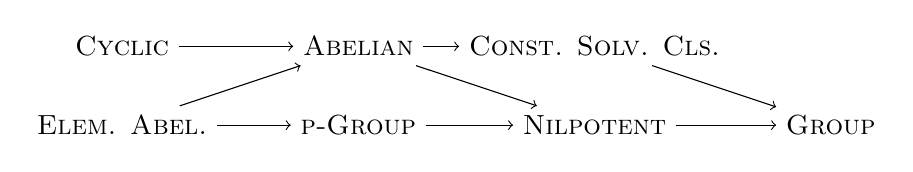
\begin{tikzpicture}[xscale=3]

      \node (e) at (0, 0) {\textsc{Elem. Abel.}};
      \node (c) at (0, 1) {\textsc{Cyclic}};
      \node (p) at (1, 0) {\textsc{p-Group}};
      \node (a) at (1, 1) {\textsc{Abelian}};
      \node (n) at (2, 0) {\textsc{Nilpotent}};
      \node (s) at (2, 1) {\textsc{Const. Solv. Cls.}};
      \node (g) at (3, 0) {\textsc{Group}};

      \path[->]
      (c) edge (a)
      (e) edge (a)
      (e) edge (p)

      (a) edge (s)
      (a) edge (n)
      (p) edge (n)

      (s) edge (g)
      (n) edge (g);
    \end{tikzpicture}
  \end{center}
\end{figure}

\section{Results}

In order to study the complexity of computing the size of the minimum generating set, we define a decision problem corresponding to this optimization problem.

\begin{definition}[\textsc{Min Gen Size($\mathcal{G}$)}]
  \mbox{}

  \textbf{Instance:} finite group $G$ (given as a Cayley table) in the class $\mathcal{G}$, natural number $k$ (given in binary).

  \textbf{Question:} Does there exist a $T \subseteq G$ such that $\gen{T} = G$ and $|T| \leq k$?
\end{definition}

Since each of the other classes of groups is a subclass of \textsc{Group}, an upper bound on the complexity of \textsc{Min Gen Size(Group)} is also an upper bound on the complexity of \textsc{Min Gen Size} for all the other subclasses.

%% TODO I can't find a copy of \cite{lsz77} online.
Previously, the \textsc{Min Gen Size(Group)} problem was known to be in $\L^2$, the class of problems decidable by a deterministic Turing machine using at most $O(\log^2 n)$ space \cite{lsz77} (see \cite[Proposition~3]{at06} for a brief description of the algorithm)
We can improve this upper bound by a more careful analysis of the $\L^2$ algorithm using the following auxiliary decision problem.

\begin{definition}[\textsc{Membership($\mathcal{G}$)}]
  \mbox{}

  \textbf{Instance:} finite group $G$ (given as a Cayley table) in the class $\mathcal{G}$, finite set $S \subset G$, group element $v \in G$.

  \textbf{Question:} Is $v \in \gen{S}$?
\end{definition}

\begin{lemma}\label{lem:membershipinl}
  $\textsc{Membership(Group)} \in \L$.
\end{lemma}
\begin{proof}
  Since $\textsc{Membership(Group)} \in \SL$ \cite[Section~3]{bm89}, and $\SL = \L$ \cite{reingold08}, the lemma follows.
\end{proof}

Upper bounds on the complexity of \textsc{Membership($\mathcal{G}$)} for several subclasses of \textsc{Group} are explored in \cite{bklm01}.
%We use the logarithmic space algorithm for this problem to give a simple $\GC(\log^2 n, \L)$ algorithm for \textsc{Min Group Gen}.

Before providing the general algorithms for computing the size of the minimum generating set for classes of groups, we require one algebraic lemma which bounds the size of the minimum generating set of any finite group.

\begin{lemma}\label{lem:log}
  If $G$ is a finite group of order $n$ then the minimum size of a generating set is at most $\log n$.
\end{lemma}
%% The previous attempted proof was from
%% \url{http://math.stackexchange.com/a/226938/29369}. This proof is from
%% \url{http://www.imsc.res.in/~arvind/notes.pdf}.
\begin{proof}
  Suppose $m$ is the size of the minimum generating set.
  Let $H_0 = \gen{e}$, where $e$ is the identity element in $G$.
  For each $i \in \{1, \dotsc, m\}$, let $H_i = \gen{H_{i - 1}, x_i}$ where $x_i \in (G \setminus H_{i - 1})$.
  Such an $x_i$ must exist for each $i$ because otherwise we would have some set $H_j$, of size less than $m$, which generates the group $G$; this violates the hypothesis that $m$ is the minimum size of a generating set for $G$.

  Now, for each $i \in \{1, \dotsc, m\}$, we have $x_i \neq e$, by construction.
  Furthermore, the cosets $x_i \gen{H_{i - 1}}$ and $e \gen{H_{i - 1}}$ are disjoint.
  If we suppose to the contrary that there is some element $y \in e \gen{H_{i - 1}} \cap x_i \gen{H_{i - 1}}$, then $y = x_i h$ for some $h \in \gen{H_{i - 1}}$, which implies $x_i = yh^{-1}$, and hence $x_i \in H_{i - 1}$.
  This is a contradiction with the hypothesis that $x_i \in (G \setminus H_{i - 1})$.
  Therefore $|\gen{H_i}| \geq 2 |\gen{H_{i - 1}}|$.
  By induction, $|G| = |\gen{H_m}| \geq 2^m$, which implies $m \leq \log |G| = \log n$.
\end{proof}

This lemma allows us to consider, without loss of generality, only inputs $\pair{G}{k}$ such that $k \leq \log n$.

\begin{theorem}\label{thm:mingengc}
  $\textsc{Min Gen Size(Group)} \in \GC(\log^2 n, \L)$.
\end{theorem}
\begin{proof}
  The algorithm proceeds as follows on input $\pair{G}{k}$, where $G$ is a group of order $n$:
  \begin{enumerate}
  \item Nondeterministically guess a subset $S \subseteq G$ of cardinality at most $k$.
  \item Accept if and only if for all $v \in G$, $\triple{G}{S}{v} \in \textsc{Membership(Group)}$.
  \end{enumerate}

  First we prove that this algorithm uses $O(\log^2 n)$ nondeterministic bits and $O(\log n)$ space.
  The size of each group element, represented as number in binary, is $\log n$.
  By \autoref{lem:log}, we assume without loss of generality that the size of the minimum generating set for a group of order $n$ is at most $\log n$, so $k$ must be at most $\log n$.
  Therefore the total number of nondeterministic bits required to guess $S$ is $O(\log^2 n)$.
  Iterating over all elements of $G$ requires $O(\log n)$ space to keep track of the current element in the iteration.
  Since $\textsc{Membership(Group)} \in \L$ by \autoref{lem:membershipinl}, deciding whether $\triple{G}{S}{v} \in \textsc{Membership(Group)}$ uses at most $O(\log n)$ space.
  Therefore the total space required for this algorithm (other than the read-only input and read-only nondeterministic bits) is $O(\log n)$.

  Next we show that the algorithm correctly decides the problem.
  Suppose $\pair{G}{k} \in \textsc{Min Gen Size(Group)}$, so there exists a $T \subseteq G$ such that $|T| \leq k$ and $\gen{T} = G$.
  One of the sets $S$ of cardinality at most $k$ that the algorithm guesses will equal $T$, since $|T| \leq k$.
  For all elements $v \in G$, we have $v \in \gen{T}$ since $\gen{T} = G$.
  Hence the (correct) algorithm for \textsc{Membership(Group)} will accept for all $v \in G$, and the overall algorithm will accept.
  For the converse, suppose the algorithm accepts the input $\pair{G}{k}$.
  This occurs exactly when it has guessed a set $S$ of cardinality at most $k$ such that all elements $v$ in $G$ are members of the subgroup generated by $S$.
  Thus $S$ is a generating set for $G$ of cardinality at most $k$, so $\pair{G}{k} \in \textsc{Min Gen Size(Group)}$.
\end{proof}

This improves the previous upper bound, $\L^2$, because
\begin{equation*}
  \GC(\log^2 n, \L) \subseteq \NL \cap \GC(\log^2 n, \NC^2) \subseteq \NL \cup \GC(\log^2 n, \NC^2) \subseteq \L^2.
\end{equation*}
(In the first inclusion we use the fact that $\L \subseteq \NL \subseteq \NC^2$.
In the last inclusion we use Savitch's Theorem and the fact that $\GC(\log^d n, \NC^k) \subseteq \L^{\max{(d, k)}}$ \cite[Lemma~3.1]{wolf94}.)

\begin{theorem}
  \mbox{}
  \begin{enumerate}
  \item Each of the problems
    \begin{itemize}
    \item \textsc{Min Gen Size(Constant Solvability Class)},
    \item \textsc{Min Gen Size(Abelian)},
    \item \textsc{Min Gen Size(Elementary Abelian)}, and
    \item \textsc{Min Gen Size(Cyclic)}
    \end{itemize}
    is in $\GC(\log^2 n, \FOLL)$.
  \item $\textsc{Min Gen Size(Nilpotent)} \in \GC(\log^2 n, \FOLL^2)$.
  \end{enumerate}
\end{theorem}
\begin{proof}
  \mbox{}
  \begin{enumerate}
  \item
    We know that the membership problem for each of these classes of groups is in \FOLL{} by \cite[Section~3]{bklm01}.
    A slight modification of the algorithm from \autoref{thm:mingengc} can be used to show that each of these problems is in $\GC(\log^2 n, \FOLL)$.
    After nondeterministically guessing a set $S$, instead of iterating over each element of the group in logarithmic space, we use in parallel $n$ instances of the \FOLL{} circuit which decides the membership problem and compute the conjunction of the output of each of the instances for one additional layer of depth and a $O(n)$ increase in the size of the circuit.
    Since the size of the circuit remains polynomial in $n$ and the depth remains $O(\log \log n)$, we have shown $\textsc{Min Gen Size(Cyclic)} \in \GC(\log^2 n, \FOLL)$.
  \item The same argument applies, except using the fact that the membership problem for nilpotent groups is in $\FOLL^2$ \cite[Corollary~3.12]{bklm01}. \qedhere
  \end{enumerate}
\end{proof}
%% Observe that even though, for example, $\textsc{Membership(Cyclic)} \in \L \cap \FOLL$, we show that \textsc{Min Gen Size(Cyclic)} is in
%% \begin{equation*}
%%   \GC(\log^2 n, \L) \cap \GC(\log^2 n, \FOLL)
%% \end{equation*}
%% instead of
%% \begin{equation*}
%%   \GC(\log^2 n, \L \cap \FOLL),
%% \end{equation*}
%% for syntactic reasons (the second step in the algorithm from \autoref{thm:mingengc} is either a logarithmic space Turing machine procedure or a $\FO(\log \log n)$ procedure, but not both simultaneously).

In \cite{at06}, the authors provide a polynomial time conjunctive truth-table reduction from \textsc{Min Gen Size(Nilpotent)} to \textsc{Min Gen Size(Elementary Abelian)} via \textsc{Min Gen Size(p-Group)}.
They note that since there exists a deterministic polynomial time algorithm for \textsc{Min Gen Size(Elementary Abelian)}, there is one for each of the others as well.
This result also implies a polynomial time algorithm for all subclasses of the the class of finite nilpotent groups.
A more detailed presentation of the complete proof is given in \autoref{app:p}.

\begin{theorem}[{\cite[Theorem~7]{at06}}]
  Each of the problems
  \begin{itemize}
  \item \textsc{Min Gen Size(Nilpotent)},
  \item \textsc{Min Gen Size(p-Group)},
  \item \textsc{Min Gen Size(Abelian)},
  \item \textsc{Min Gen Size(Elementary Abelian)}, and
  \item \textsc{Min Gen Size(Cyclic)}
  \end{itemize}
  is in \P.
\end{theorem}

For cyclic groups, the size of the minimum generating set is always 1, so the problem is uninteresting.

\begin{theorem}
  $\textsc{Min Gen Size(Cyclic)} \in \NC^0$.
\end{theorem}

The attentive reader may wonder if we can improve the upper bound given in the previous sections for computing \textsc{Min Gen Size} for elementary abelian groups, which, like cyclic groups, are very highly structured.
The elementary abelian groups are isomorphic to the additive group $(\mathbb{Z}/p\mathbb{Z})^m$ for some prime $p$ and some non-negative integer $m$.
The size of the minimum generating set for an elementary abelian group of order $p^m$ is $m$: each of the $m$ elements has the generator for $\mathbb{Z}/p\mathbb{Z}$ in exactly one coordinate and the identity in each of the other coordinates.
Hence we have reduced the problem of computing the size of the minimum generating set to the problem of computing the function $p^m \mapsto m$, where $p^m$ is given in unary.


%% Algorithm for computing prime powers: http://mathoverflow.net/questions/106313/algorithm-for-detecting-prime-powers
%%
%% Algorithm for computing perfect powers: http://cr.yp.to/papers/powers.pdf
\begin{lemma}
  The function $f(n) = m$, where $n = p^m$, $n$ is given in unary, $p$ is a prime, and $m$ is a non-negative integer is computable by an \NC{} circuit family.
\end{lemma}
\begin{proof}
  The following algorithm computes $m$ from the (unary) input $1^n$ where $n = p^m$ for some prime $p$ and some integer $m$.
  Here, \textsc{Unary Primes} is the set of all prime numbers expressed as unary integers.
  \begin{enumerate}
  \item Nondeterministically choose an $m'$ between 0 and $\log n$, expressed in unary.
  \item Let $p' = \sqrt[m']{n}$.
  \item Output $m'$ if and only if $p' \in \textsc{Unary Primes}$.
  \end{enumerate}
  The first step requires $\log n$ bits of nondeterminism.
  In the second step, computing the $m'$th root of $n$ can be done in \NC{}, since the input is given in unary.
  In the third step, deciding if a number is prime can be done in \NC{}, again since the input is given in unary, by using an efficient deterministic polynomial time algorithm like the AKS primality test \cite{aks04}.
  If the input is properly formatted (that is, if it is a prime power), then there will be exactly one $p'$ which is a prime number, by the Fundamental Theorem of Arithmetic.
  Therefore this algorithm will certainly halt and output an $m'$ such that $n = {p'}^{m'}$.
  Hence this is a correct \NC{} algorithm which computes $m$ and $p$ from $p^m$ using $O(\log n)$ bits of nondeterminism.

  Since $\GC(\log n, \NC) = \NC$ \cite[Theorem~2.3]{wolf94}, we conclude that there is an \NC{} circuit family computing this function.
\end{proof}

From the discussion preceding the lemma, we immediately get the following theorem.

\begin{theorem}\label{thm:eainnc}
  $\textsc{Min Gen Size(Elementary Abelian)} \in \NC$.
\end{theorem}

Finally, we show some negative completeness results, providing more specific upper bounds for the complexity of computing the size of the minimum generating set of a group.
Any decision problem in \FOLL{} (or $\FOLL^2$) cannot be hard under $\AC^0$ many-one reductions for any complexity class which contains $\textsc{Parity}$ \cite[Section~2.2]{bklm01}.
This is true even when the circuit is augmented with a polylogarithmic number of nondeterministic gates \cite[Section~4]{ctw10}.
This gives an immediate improvement to the upper bound of all the problems shown in the previous section to be in $\GC(\log^2 n, \FOLL)$ (or $\GC(\log^2 n, \FOLL^2)$).

\begin{theorem}
  None of the decision problems
  \begin{itemize}
  \item \textsc{Min Gen Size(Nilpotent)},
  \item \textsc{Min Gen Size(p-Group)},
  \item \textsc{Min Gen Size(Constant Solvability Class)},
  \item \textsc{Min Gen Size(Abelian)},
  \item \textsc{Min Gen Size(Elementary Abelian)}, or
  \item \textsc{Min Gen Size(Cyclic)}
  \end{itemize}
  are hard under $\AC^0$ many-one reductions for any complexity class containing \textsc{Parity}, specifically those in the inclusion chain
  \begin{equation*}
    \ACC^0 \subseteq \TC^0 \subseteq \NC^1 \subseteq \L \subseteq \NL \subseteq (\LOGCFL \cup \DET).
  \end{equation*}
\end{theorem}

\section{Future work}

As noted in the introduction, the (quasi)group isomorphism problem is known to be in $\GC(\log^2 n, \FOLL)$.
What is the relationship between this problem and the minimum generating set size problem for groups?

What is the precise relationship between computing the minimum generating set and computing the size of the minimum generating set?
An efficient function which computes the minimum generating set implies an efficient function which computes the size of the minimum generating set (compute the set, then compute its cardinality), so we know that the former must be at least as hard as the latter.
On the other hand, it seems unlikely that knowing the size of a minimum generating set would yield any information about the contents of such a set.

\section{About this work}

Copyright 2012 Jef{}frey Finkelstein.

This work is licensed under the Creative Commons Attribution-ShareAlike License 3.0.
Visit \mbox{\url{https://creativecommons.org/licenses/by-sa/3.0/}} to view a copy of this license.

The \LaTeX{} markup which generated this document is available on the World Wide Web at \mbox{\url{https://github.com/jfinkels/mingroupgen}}.
It is also licensed under the Creative Commons Attribution-ShareAlike License.

The author can be contacted via email at \email{jeffreyf@bu.edu}.

\bibliographystyle{plain}
\bibliography{references}

\appendix
\section{Polynomial time algorithm for finite nilpotent groups}\label{app:p}

At this point, we provide a clearer presentation of the proof of \cite[Theorem~7]{at06}.
We have split up the proof into multiple parts in order to more easily analyze their complexity.

We say \emph{$P$ is conjunctive truth-table reducible to $Q$} if there exists a function $f$ such that for all strings $x$, we have $f(x) = \langle y_1, y_2, \dotsc, y_m \rangle$ for some positive integer $m$ and $x \in P$ if and only if for all $i \leq m$, we have $y_i \in Q$.

\begin{lemma}\label{lem:sylow}
  Suppose $(G, \cdot)$ is a finite group of order $n$, where the (unique) prime factorization of $n$ is $\Pi_{i = 1}^m p_i^{e_i}$.
  Then $G$ is nilpotent if and only if $G \cong S_{p_1} \times S_{p_2} \times \dotsb \times S_{p_m}$ where each $S_{p_i}$ is the unique $p_i$-Sylow subgroup of $G$.
\end{lemma}

%% \begin{lemma}
%%   Suppose $(G, \cdot)$ and $(H, \circ)$ are groups such that $G \cong H$ and $k$ is a non-negative integer.
%%   $G$ has a generating set of size $k$ if and only if $H$ has a generating set of size $k$.
%% \end{lemma}

\begin{proposition}
  \begin{equation*}
    \textsc{Min Gen Size(Nilpotent)} \leq_{ctt}^P \textsc{Min Gen Size(p-Group)}.
  \end{equation*}
\end{proposition}
\begin{proof}
  Define the reduction by
  \begin{equation*}
    \langle (G, \cdot), k \rangle \mapsto \left\langle (S_{p_1}, k), (S_{p_2}, k), \dotsc, (S_{p_m}, k) \right\rangle
  \end{equation*}
  for all nilpotent groups $(G, \cdot)$ of order $n$ and all positive integers $k$, where the prime factorization of $n$ is $p_1^{e_1}p_2^{e_2}\dotsb p_m^{e_m}$ and $S_{p_i}$ is the unique $p_i$-Sylow subgroup of $G$.
  Observe that the output is correctly formatted because each of the Sylow subgroups is a $p$-group.

  First we show that this reduction is computable in deterministic polynomial time.
  Since the length of the input is $n^2 \log n$, the prime factorization of $n$ can be computed in deterministic polynomial time with respect to the length of the input (using, for example, the general number field sieve \cite{llmp93}).
  We know that the set of Sylow subgroups exists by \autoref{lem:sylow}.
  If $n_i = n p_i^{-e_i}$ then $S_{p_i} = \{g^{n_i} \, | \, g \in G\}$ for all $i \leq m$.
  The $n_i$th power of $g$ can be computed in logarithmic space (by iteratively computing $g$, $g^2$, $g^3$, etc.).
  Computing the set $S_{p_i}$ can therefore be computed in logarithmic space as well.
  Constructing the Cayley table of $S_{p_i}$ can be performed in constant space by simply looking up the appropriate entries in the Cayley table of the group $G$.
  The total number of clauses in the conjunction is $m$, which is the number of prime factors of $n$, which is bounded by a polynomial in $n^2 \log n$ because the number of prime factors of $n$ is less than $n$.
  Hence the reduction is polynomial time computable.

  Next we show that the reduction is correct.
  Suppose first that $\langle (G, \cdot), k \rangle \in \textsc{Min Gen Size(Nilpotent)}$, so there exists a subset of $G$, say $\{g_1, g_2, \dotsc, g_k\}$, such that $\gen{g_1, g_2, \dotsc, g_k} = G$.
  If $n_i = n p_i^{-e_i}$, as defined above, then the set $\{g_1^{n_i}, g_2^{n_i}, \dotsc, g_k^{n_i} \}$ is a generating set for $S_{p_i}$.
  So for each $i$ with $1 \leq i \leq m$, we have $\langle (S_{p_i}, \cdot), k \rangle \in \textsc{Min Gen Size(p-Group)}$.
  For the converse, suppose that each $S_{p_i}$ has a generating set of size $k$, say $\{g_{i, 1}, g_{i, 2}, \dotsc, g_{i, k}\}$.
  Let $g_j = \Pi_{i = 1}^m g_{i, j}$ for all $j$ with $1 \leq j \leq k$.
  In other words, $g_j$ is the product of all the $j$th elements in the generating sets of $S_{p_1}$, $S_{p_2}, \dotsc, S_{p_m}$.
  Since $\gen{g_1^{n_i}, g_2^{n_i}, \dotsc, g_k^{n_i}} = S_{p_i} $, we have $\gen{g_1, g_2, \dotsc, g_k} = G$.

  We have now shown a correct deterministic polynomial time conjunctive truth table reduction from \textsc{Min Gen Size(Nilpotent)} to \textsc{Min Gen Size(p-Group)}.
\end{proof}

\begin{lemma}\label{lem:decompose}
  If $(G, \cdot)$ is a finite abelian group, then there exists a finite set of cyclic groups $\{H_1, H_2, \dotsc, H_t\}$ such that $G \cong H_1 \times H_2 \times \dotsb \times H_t$.
\end{lemma}

\begin{lemma}\label{lem:factorgroup}
  If $(G, \cdot)$ is a group of order $n$ given by its Cayley table and $H < G$ then the function $\langle (G, \cdot), H \rangle \mapsto G / H$ is computable in polynomial time.
\end{lemma}
\begin{proof}
  The elements of $G / H$ can be computed by iteratively computing $g H$ for each $g \in G$.
  There are $O(n)$ such iterations, each of which requires $O(n)$ multiplications, where each multiplication requires constant time (by lookup in the Cayley table).
  Constructing the table \ldots
\end{proof}

\begin{definition}
  Suppose $(G, \cdot)$ is a group.
  The \emph{Frattini subgroup} of $G$, denoted $\Phi(G)$, is the intersection of all maximal subgroups of $G$.
\end{definition}

\begin{lemma}\label{lem:frattinip}
  Let $(G, \cdot)$ be a finite $p$-group.
  Then the function $G \mapsto \Phi(G)$ is computable in polynomial time.
\end{lemma}
\begin{proof}
  Let $G'$ be the commutator subgroup of $G$.
  We know $G' \triangleleft G$ and $G/G'$ is abelian.
  $G$ is nilpotent if and only if $G' \subseteq \Phi(G)$.
  Since $G$ is a finite $p$-group, $G$ is nilpotent.
  For any subgroup $N < G$, if $N \triangleleft G$ and $N \subseteq \Phi(G)$ then $\Phi(G / N) \cong \Phi(G) / N$.
  Hence $\Phi(G / G') \cong \Phi(G) / G'$.
  If the Cayley tables for $\Phi(G / G')$ and $G'$ can be computed in polynomial time, then so can the Cayley table for $\Phi(G)$ using this isomorphism.
  Since the table for $G'$ can be computed in polynomial time, it therefore suffices to show that the table for $\Phi(G / G')$ is computable in polynomial time.

  Since the table for $G'$ can be computed in polynomial time, so can the table for $G / G'$.
  By \autoref{lem:decompose} we can compute in polynomial time the decomposition of $G / G'$ into a product of cyclic groups $\{H_1 / G', H_2 / G', \dotsc, H_t / G'\}$, so $G / G' \cong H_1 / G' \times H_2 / G' \times \dotsb \times H_t / G'$.
  For each $j$ with $1 \leq j \leq t$, let $y_jG'$ be the element in $G / G'$ which generates $H_j / G'$, and suppose the order of $y_jG'$ is $p^{c_j}$ for some non-negative integer $c_j$.
  We know the order of $y_jG'$ must be a power of $p$ because the order of $G$ is a prime power.
  Since the group is given as a Cayley table, we can compute the generator of a cyclic group in polynomial time by iterating over each element and testing whether it is a generator.

  We know $\Phi(G / G') \cong \Phi(H_1 / G') \times \Phi(H_2 / G') \times \dotsb \times \Phi(H_t / G')$.
  Since each factor group $H_j / G'$ is a cyclic group of prime power order, it has a unique maximal proper subgroup, specifically the subgroup $\gen{y_j^pG'}$.
  Therefore, by definition of the Frattini subgroup, $\Phi(H_j / G') = \gen{y_j^pG'}$ for all $j$ with $ 1 \leq j \leq t$.
  Working our way back through the isomorphisms, we find that $\Phi(G / G') = \gen{y_1^pG', y_2^pG', \dotsc, y_t^pG'}$, and hence $\Phi(G) = \gen{y_1^p, y_2^p, \dotsc, y_t^p, G'}$.
  Since we can compute each generator $y_j$ in polynomial time, since we can compute $y_j^p$ in polynomial time, and since $t$ is bounded by $O(n)$, the size of $\Phi(G)$ is polynomial in $n$.
\end{proof}

\begin{proposition}
  \begin{equation*}
    \textsc{Min Gen Size(p-Group)} \leq_m^P \textsc{Min Gen Size(Elementary Abelian)}.
  \end{equation*}
\end{proposition}
\begin{proof}
  Define the reduction by
  \begin{equation*}
    \langle (G, \cdot), k \rangle \mapsto \langle (G / \Phi(G), \cdot), k \rangle
  \end{equation*}
  for all $p$-groups $G$ of order $n$ and all positive integers $k$, where $\Phi(G)$ is the Frattini subgroup of $G$.
  By \autoref{lem:frattinip}, the Cayley table of $\Phi(G)$ is computable in polynomial time.
  By \autoref{lem:factorgroup}, the Cayley table of $G / \Phi(G)$ is computable in polynomial time.
  Hence the reduction is polynomial time computable.

  Suppose $\langle (G, \cdot), k \rangle \in \textsc{Min Gen Size(p-Group)}$, so $G$ has a generating set of size at most $k$, say $\{g_1, g_2, \dotsc, g_k\}$.
  Then $\{g_1\Phi(G), g_2\Phi(G), \dotsc, g_k\Phi(G)\}$ is a generating set for $G / \Phi(G)$ of size at most $k$.
  For the converse suppose $\langle (G / \Phi(G), \cdot), k \rangle \in \textsc{Min Gen Size(Elementary Abelian)}$, so $G / \Phi(G)$ has a generating set of size at most $k$, say $\{g_1\Phi(G), g_2\Phi(G), \dotsc, g_k\Phi(G)\}$.
  If we let $H = \gen{g_1, g_2, \dotsc, g_k}$, then $H \Phi(G) = G$.
  Since $\Phi(G)$ is a set containing only nongenerators for $G$, we have $H = G$.
  Therefore $G$ has a generating set of size at most $k$.
  This concludes the proof.
\end{proof}

\begin{lemma}
  $\textsc{Min Gen Size(Elementary Abelian)} \in \P$.
\end{lemma}
\begin{proof}
  Every elementary abelian group is isomorphic to $(\mathbb{Z} / p\mathbb{Z})^m$ where $p$ is a prime number and $m$ is a non-negative integer.
  The minimum generating set for $\mathbb{Z} / p\mathbb{Z}$ is $\{1\}$, so the minimum generating set for $(\mathbb{Z} / p\mathbb{Z})^m$ is
  \[
  \{(1, 0, \dotsc, 0), (0, 1, 0, \dotsc, 0), \dotsc, (0, \dotsc, 0, 1)\}.
  \]
  Therefore the size of the minimum generating set for every elementary abelian group is $m$.

  On input $\langle (G, \cdot), k \rangle$, the polynomial time algorithm computes $m$, then compares that with $k$.
  To compute $m$, determine the order of the group $n$ and compute its factorization, which can be done in polynomial time when the input is given as a Cayley table (using, for example, the general number field sieve \cite{llmp93}).
\end{proof}

\begin{theorem}
  $\textsc{Min Gen Size(Nilpotent)} \in \P$.
\end{theorem}
\begin{proof}
  Since a many-one reduction implies a conjunctive truth table reduction, we have
  \begin{equation*}
    \textsc{Min Gen Size(Nilpotent)} \leq_{ctt}^P \textsc{Min Gen Size(p-Group)},
  \end{equation*}
  and
  \begin{equation*}
    \textsc{Min Gen Size(p-Group)} \leq_{ctt}^P \textsc{Min Gen Size(Elementary Abelian)}.
  \end{equation*}
  Since polynomial time conjunctive truth table reductions compose this implies
  \begin{equation*}
    \textsc{Min Gen Size(Nilpotent)} \leq_{ctt}^P \textsc{Min Gen Size(Elementary Abelian)}.
  \end{equation*}
  Since $\textsc{Min Gen Size(Elementary Abelian)} \in \P$ and $\P$ is closed under polynomial time conjunctive truth table reductions, $\textsc{Min Gen Size(Nilpotent)} \in \P$.
\end{proof}


\end{document}
